\documentclass[a4paper]{article}

% Packages
\usepackage{booktabs} % For professional looking tables like \toprule, \midrule, \bottomrule
\usepackage{array}    % For complex table column specifications
\usepackage{float}    % For better figure placement control [H]
\usepackage{geometry}
\geometry{left=2cm, right=2cm, top=2.54cm, bottom=2.54cm}
\usepackage{graphicx, hyperref, setspace, amsmath, amssymb, titlesec, fancyhdr, multicol, parskip, indentfirst, etoolbox, caption, cite, hyperref, xcolor}

\usepackage{subcaption} % Add to preamble

\usepackage{hyperref}
\hypersetup{
    colorlinks=true,
    linkcolor=blue,
    filecolor=magenta,
    urlcolor=cyan,
    pdftitle={Heart Sound Classification Report},
    pdfpagemode=FullScreen,
    }

\urlstyle{same}

% Title Formatting
\titleformat{\section}{\centering\large\scshape}{\thesection}{1em}{}
\titleformat{\subsection}{\normalsize\bfseries}{\thesubsection.}{1em}{}
\setstretch{1.0} % Keep single spacing
\setlength{\parskip}{6pt} % Space between paragraphs
\titlespacing{\section}{0pt}{6pt}{6pt}
\titlespacing{\subsection}{0pt}{6pt}{6pt}
\titlespacing{\subsubsection}{0pt}{6pt}{6pt}

% Document Title
\title{
    \textbf{Heart Sound Classification: A Deep Learning Approach Using CNN-RNN Architectures with Attention}
}
\author{Mahla Entezari}

\date{} % No date
\captionsetup{labelfont={small,sc}, textfont={small,sc}}
% Section Numbering
% Define numbering format
\renewcommand{\thesection}{\Roman{section}.}
\renewcommand{\thesubsection}{\textit{\Alph{subsection}.}}
\renewcommand{\thesubsubsection}{\textit{\arabic{subsubsection}.}}
\renewcommand{\thetable}{\Roman{table}} % Set table numbering to Roman
\renewcommand{\thefigure}{\Roman{figure}} % Number figures in Roman numerals

% Make titles italic as well
\titleformat{\subsection}{\normalfont\large\itshape}{\thesubsection}{1em}{}
\titleformat{\subsubsection}{\normalfont\itshape}{\thesubsubsection}{1em}{}

% Fancy Header Configuration
\pagestyle{fancy}
\fancyhf{} % Clear all header/footer fields
\fancyhead[C]{\textbf{Heart Sound Classification Report}} % Custom header for your report

\begin{document}

\maketitle
\vspace{-1.5cm}

% Authors Block
\begin{center}
    \textit{\\Shahid Beheshti University}\\
    \textit{Tehran, Iran}\\
    \textit{MahlaEntezari.sbu@gmail.com}\\
    \date{December 2024}
    \vfill
\end{center}

\singlespacing
\setlength{\parskip}{6pt}
\setlength{\parindent}{0.5cm}
\setlength{\columnsep}{0.5cm}

% Abstract (single-column)
\begin{abstract}
This report details a deep learning project focused on classifying heart sounds into five distinct categories: Normal, Murmur, Extra Heart Sound, Artifact, and Extrasystole. The methodology involves comprehensive audio preprocessing, including wavelet denoising, resampling, and segmentation. Mel-Frequency Cepstral Coefficients (MFCCs) are extracted as key features. A hybrid Convolutional Neural Network (CNN) and Recurrent Neural Network (RNN) framework is employed, where the CNN extracts short-term patterns, and various RNN architectures (Simple RNN, LSTM, Bi-LSTM, GRU, and a conceptual xLSTM) model temporal dependencies. Furthermore, a soft attention mechanism is integrated with the LSTM to enhance performance and interpretability. The models are trained using CrossEntropyLoss and the Adam optimizer, with performance evaluated through accuracy, precision, recall, F1-score, and confusion matrices. Results indicate that advanced RNNs, particularly Bi-LSTM and LSTM with attention, achieve better performance compared to Simple RNN, demonstrating the importance of capturing complex temporal patterns and focusing on salient audio segments in heart sound classification. Challenges related to class imbalance are also discussed.
\end{abstract}

\begin{multicols}{2}

\section{Introduction}
Accurate and automated classification of heart sounds is a critical step towards early diagnosis and monitoring of cardiovascular diseases. Phonocardiography, the recording of heart sounds, provides non-invasive insights into cardiac function. However, manual interpretation of these sounds by medical professionals is time-consuming and requires extensive expertise. The advent of deep learning offers a powerful avenue to automate this process, enabling more efficient and accessible diagnostic tools.

This project aims to develop a robust deep learning model for classifying heart sounds into five predefined categories: Normal, Murmur, Extra Heart Sound (Extrahls), Artifact, and Extrasystole. These classifications are crucial for distinguishing between healthy heart sounds and various pathological conditions or external interferences. The task is challenging due to the inherent variability of heart sounds, the presence of background noise, and the often subtle differences between pathological conditions.

The dataset used for this project is the Pascal Heart Sound Dataset, which combines recordings from public sources (iStethoscope Pro - Dataset A) and hospital environments (DigiScope - Dataset B). This diverse collection of audio data provides a realistic foundation for training and evaluating a robust classification system.

The methodology adopted in this project encompasses several key stages:
\begin{enumerate}
    \item \textbf{Audio Preprocessing:} Raw audio recordings are cleaned and standardized to ensure consistency and quality.
    \item \textbf{Feature Extraction:} Relevant features that capture the discriminative characteristics of heart sounds are derived from the preprocessed audio.
    \item \textbf{Model Architecture Design:} A hybrid deep learning framework, combining Convolutional Neural Networks (CNNs) and various Recurrent Neural Networks (RNNs), is designed to effectively learn both spatial and temporal patterns in the audio features.
    \item \textbf{Model Training and Evaluation:} The designed models are trained on the prepared data, and their performance is rigorously evaluated using standard classification metrics.
    \item \textbf{Attention Mechanism Integration:} A soft attention mechanism is incorporated to enhance the model's ability to focus on critical segments of the heart sound.
\end{enumerate}

Beyond the practical application, this report also briefly touches upon theoretical concepts relevant to advanced deep learning architectures, such as Variational Autoencoders (VAEs) and specialized LSTM variants like xLSTM. Understanding these foundational and advanced concepts is essential for appreciating the complexities and potential of contemporary neural network designs, which inform the architectural choices made in this heart sound classification task.

\subsection{Theoretical Background: Advanced Neural Network Concepts}
To provide context for the advanced architectures explored, it's beneficial to briefly discuss key concepts in deep learning, some of which (like xLSTM) are conceptually part of this project's scope.

\subsubsection{Variational Autoencoders (VAEs)}
Variational Autoencoders (VAEs) are powerful generative models that learn a latent representation of data. They consist of an encoder (that maps input to a probabilistic latent space) and a decoder (that reconstructs input from latent samples). Sampling from the latent distribution $q(z|x)$ within VAEs presents two main challenges:
\begin{enumerate}
    \item \textbf{Non-Differentiability:} Direct sampling, being a stochastic operation, breaks the flow of gradients during backpropagation. This makes it impossible to directly train the encoder using gradient-based methods, as the gradients cannot pass through the random sampling step.
    \item \textbf{High Variance Gradients:} Even if approximations or alternative gradient estimation techniques (like REINFORCE) are used, the resulting gradients can suffer from high variance. This leads to unstable and inefficient training, requiring a large number of samples or complex variance reduction techniques.
\end{enumerate}
The \textbf{reparameterization trick} elegantly solves these problems. Instead of directly sampling $z$ from $q(z|x)$ (which is typically assumed to be a Gaussian distribution), it redefines the sampling process as:
$$ z = \mu(x) + \sigma(x) \cdot \epsilon $$
where $\mu(x)$ and $\sigma(x)$ are outputs of the encoder network (representing the mean and standard deviation of the latent distribution, respectively), and $\epsilon$ is a random noise vector sampled from a standard normal distribution (e.g., $N(0, 1)$). This transformation shifts the stochasticity from the sampling layer to an input noise variable, making the operation differentiable. Consequently, gradients can flow smoothly through $\mu(x)$ and $\sigma(x)$, enabling effective backpropagation and stable, lower-variance gradient estimates for training VAEs.

The hyperparameter \textbf{$\beta$} in VAEs, particularly in $\beta$-VAEs, controls the balance between reconstruction accuracy and the disentanglement of latent representations:
\begin{itemize}
    \item \textbf{Higher $\beta$ (>1):} Emphasizes the Kullback-Leibler (KL) divergence term in the VAE's loss function. This encourages the latent distribution $q(z|x)$ to be closer to the prior distribution (often a standard normal), promoting more disentangled latent representations. However, this may come at the cost of reduced reconstruction quality, as the model prioritizes a structured latent space over precise data reconstruction.
    \item \textbf{Lower $\beta$ (<1):} Places more weight on the reconstruction loss, prioritizing accurate data reconstruction. This allows the model to capture more detailed information from the input, but may result in less disentangled or interpretable latent factors, as the latent space is not strongly regularized.
    \item \textbf{$\beta = 1$:} Represents the standard VAE formulation, balancing both reconstruction accuracy and disentanglement. It provides a trade-off that aims to reconstruct data well while maintaining a reasonably structured latent space.
\end{itemize}

\subsubsection{Peephole Connections in LSTMs}
Peephole connections are an enhancement to the standard Long Short-Term Memory (LSTM) network architecture. In a traditional LSTM, the gate mechanisms (input, forget, and output gates) control the flow of information into and out of the cell state, but they only receive input from the current input and the previous hidden state. Peephole connections allow these gates to directly "peek" at or access the cell state (the internal memory of the LSTM cell).

This direct access enhances the network's ability to regulate information flow and maintain the cell state more effectively. For example, the forget gate can decide whether to keep or discard information in the cell state based not only on the new input and previous hidden state but also on the current contents of the cell state itself. This enables better control over forgetting and output mechanisms, potentially improving the learning of long-term temporal dependencies, especially in complex sequence modeling tasks.

However, peephole connections introduce additional parameters to the LSTM cell, increasing the computational complexity of the model. This increased complexity also carries a higher risk of overfitting, particularly in scenarios with limited training data. Moreover, for tasks with simpler temporal structures where standard LSTMs already perform adequately, peephole connections may offer minimal benefits and might not justify the added complexity. Therefore, while they can enhance performance in specific complex scenarios, their advantage is not universal.

\subsubsection{xLSTM}
\textbf{xLSTM} is conceptualized as an enhanced variant of the standard Long Short-Term Memory (LSTM) network, incorporating several advanced features to address limitations in capturing long-term dependencies and improving training stability. While specific implementations may vary, typical enhancements in advanced LSTM concepts like xLSTM include:
\begin{itemize}
    \item \textbf{Attention Mechanisms:} These allow the network to dynamically weigh the importance of different parts of the input sequence, enabling it to focus on the most relevant information when making predictions.
    \item \textbf{Residual Connections:} By creating shortcuts that bypass one or more layers, residual connections help in preserving gradient flow, mitigating the vanishing gradient problem, and enabling the training of much deeper networks.
    \textbf{Bidirectional Processing:} This involves processing the input sequence in both forward and backward directions, allowing the network to incorporate context from both past and future states simultaneously.
\end{itemize}
Compared to standard LSTMs, architectures like xLSTM offer greater expressiveness and stability during training. They effectively address issues like vanishing gradients (through residual connections) and limited context comprehension (through attention and bidirectionality), which can be problematic for very long sequences in standard LSTMs. These advancements make xLSTM more adept at handling complex sequential tasks, such as natural language processing and time-series forecasting, by providing a more powerful and flexible framework for learning intricate temporal patterns.

\section{Dataset Description}
The core data for this project is derived from the Pascal Heart Sound Dataset. This dataset is compiled from two main sources: Dataset A, which includes public recordings from the iStethoscope Pro application, and Dataset B, comprising hospital recordings from DigiScope. The combination of these sources provides a diverse and comprehensive collection of heart sound recordings, critical for training a robust classification model.

\subsection{Data Loading and Initial Structure}
Audio files, specifically \texttt{.wav} files, are organized into folders corresponding to their respective labels: \texttt{artifact}, \texttt{extrahls}, \texttt{extrastole}, \texttt{murmur}, and \texttt{normal}. These files were downloaded via \texttt{kagglehub}  and loaded into pandas DataFrames. A custom function, \texttt{load\_audio\_from\_folder}, was developed to iterate through these directories, load each \texttt{.wav} file using \texttt{librosa}, and extract initial metadata such as filename, raw signal data, sampling rate, duration, and the assigned label.

The loaded data is then concatenated into a single master DataFrame, \texttt{df}, which serves as the primary data source for subsequent preprocessing and feature extraction steps. Each row in this DataFrame represents a single heart sound recording. An example of the initial DataFrame structure for 'normal' sounds can be seen from the notebook output.

\subsection{Key Characteristics and Initial Observations}
Understanding the characteristics of the raw audio data is crucial for designing effective preprocessing strategies.

\begin{itemize}
    \item \textbf{Varied Sampling Rates:} The dataset contains recordings with different sampling rates (e.g., 4000 Hz, 44100 Hz). This necessitates a resampling step to ensure all audio signals are processed consistently.
    \item \textbf{Variable Durations:} The heart sound recordings vary significantly in length, ranging from less than a second to over 27 seconds. The distribution of these durations is visualized in Figure~\ref{fig:audio_durations}, showing a concentration of shorter recordings but a tail extending to longer ones. This variability requires a segmentation or padding strategy to achieve fixed-size inputs for neural networks.
    \item \textbf{Presence of Noise:} As medical recordings, heart sounds often contain background noise (e.g., breathing or ambient sounds)  that can obscure the actual heart sound components. This indicates the need for a denoising procedure.
    \item \textbf{Class Imbalance:} The distribution of labels across the five heart sound categories is not uniform, as illustrated in Figure~\ref{fig:label_distribution}. 'Normal' sounds constitute the majority class, significantly outnumbering 'murmur', 'extrasystole', 'artifact', and 'extrahls' (Extra Heart Sounds). This imbalance is a critical challenge, as models may develop a bias towards the majority class, leading to poor performance on minority classes. Strategies like stratified splitting are essential, and techniques to mitigate imbalance (e.g., weighted loss, oversampling) might be considered in future work.
\end{itemize}

\begin{minipage}{\columnwidth}
    \centering
    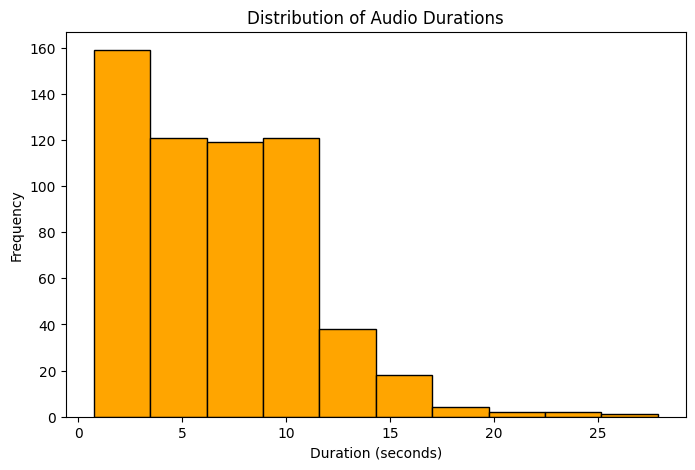
\includegraphics[width=0.9\textwidth]{output-3.png}
    \captionof{figure}{Distribution of Audio Durations.}
    \label{fig:audio_durations}
\end{minipage}

\noindent \textbf{\ref{fig:audio_durations}:}
Figure~\ref{fig:audio_durations} presents a histogram illustrating the distribution of audio durations (in seconds) across all heart sound recordings in the dataset. The x-axis represents the duration in seconds, and the y-axis indicates the frequency (count) of recordings within each duration bin. The plot reveals that a large number of recordings are relatively short, with a prominent peak around 2-4 seconds. The frequency gradually decreases as duration increases, with a long tail extending to recordings as long as 27 seconds. This variability in duration necessitates a standardized approach for inputting audio signals into the neural network, such as truncation or padding, to ensure uniform input dimensions. The choice of a fixed duration (e.g., 4 seconds) must consider this distribution to minimize loss of information or excessive padding.

\vspace{1em}

\begin{minipage}{\columnwidth}
    \centering
    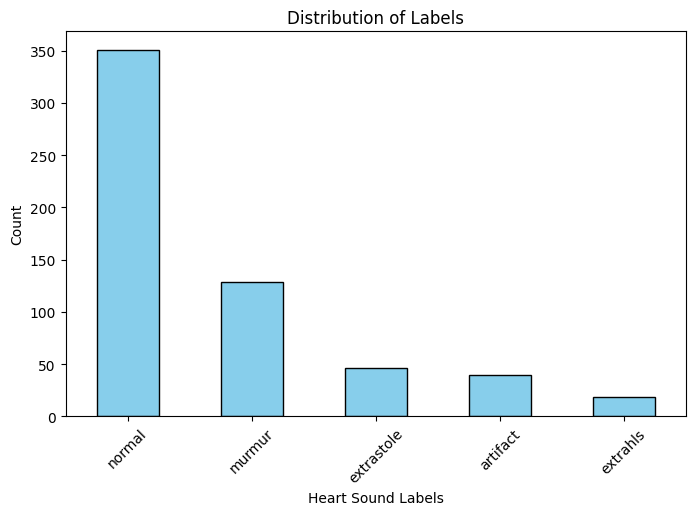
\includegraphics[width=0.9\textwidth]{output-4.png}
    \captionof{figure}{Distribution of Heart Sound Labels.}
    \label{fig:label_distribution}
\end{minipage}

\noindent \textbf{\ref{fig:label_distribution}:}
Figure~\ref{fig:label_distribution} displays a bar chart showing the distribution of heart sound labels across the dataset. The x-axis lists the five distinct heart sound labels: 'normal', 'murmur', 'extrasystole', 'artifact', and 'extrahls'. The y-axis represents the count of recordings for each label. The chart clearly indicates a significant class imbalance. 'Normal' heart sounds constitute the vast majority of the dataset, with a count exceeding 350. In contrast, 'murmur' is the next most frequent but has less than 150 instances, while 'extrasystole', 'artifact', and 'extrahls' are minority classes, with 'extrahls' having the fewest instances (approximately 20). This severe imbalance poses a challenge for classification models, as they may become biased towards the majority 'normal' class, leading to poor recall and precision for the underrepresented categories. Stratified sampling during data splitting is crucial to maintain these proportions, but additional techniques may be required during training to address this issue effectively.

\section{Preprocessing and Feature Extraction}
Effective preprocessing and feature extraction are paramount for transforming raw audio signals into a format suitable for deep learning models, especially given the diverse and noisy nature of heart sound recordings.

\subsection{Denoising}
Heart sound recordings often suffer from various forms of background noise, which can interfere with the accurate identification of cardiac events. To mitigate this, a wavelet-based denoising technique was applied.
\begin{itemize}
    \item \textbf{Wavelet Decomposition:} The raw audio signal is decomposed into different frequency sub-bands using the `db4` wavelet at a specified level (e.g., level 2, as commonly used for audio processing). This process generates a set of wavelet coefficients representing the signal's information at various scales and frequencies (\texttt{pywt.wavedec}).
    \item \textbf{Thresholding:} Noise components typically have smaller coefficients than significant signal components. A universal threshold is calculated based on the median absolute deviation (MAD) of the detail coefficients, which is robust to outliers. Soft thresholding (\texttt{pywt.threshold(c, threshold, mode='soft')}) is then applied, shrinking coefficients below the threshold towards zero. This effectively suppresses noise while preserving important signal features.
    \item \textbf{Wavelet Reconstruction:} The thresholded coefficients are then used to reconstruct the denoised signal (\texttt{pywt.waverec}).
\end{itemize}
This denoising step ensures that the subsequent feature extraction process focuses on the actual heart sounds rather than extraneous noise.

\subsection{Resampling}
Audio recordings in the dataset come with different original sampling rates. To ensure uniformity and compatibility with the deep learning model, all signals are resampled to a consistent target sampling rate of 4000 Hz.
\begin{itemize}
    \item \textbf{Standardization:} Resampling converts all audio clips to a common sampling frequency, which is crucial for creating features of consistent dimensions and for models that expect fixed input rates.
    \item \textbf{Efficiency:} A lower sampling rate (4 kHz) is chosen to reduce computational load without significant loss of information for heart sound analysis, as most relevant cardiac frequencies are below this Nyquist frequency.
\end{itemize}
The \texttt{librosa.load} function is initially used with \texttt{sr=None} to preserve the original sampling rate, and then \texttt{scipy.signal.resample} is used to convert to the target \texttt{sr}.

\subsection{Segmentation and Padding}
Deep learning models typically require inputs of fixed dimensions. Given the variable durations of heart sound recordings, a standardization step is necessary.
\begin{itemize}
    \item \textbf{Fixed Length:} All audio clips are standardized to a desired length (e.g., 4 seconds). This length is chosen as a trade-off, aiming to capture sufficient temporal context while minimizing excessive padding or truncation of longer signals.
    \item \textbf{Padding:} For recordings shorter than the desired length, zero-padding is applied to the end of the signal (\texttt{np.pad}). This ensures that all inputs have the same temporal dimension.
    \item \textbf{Truncation:} For recordings longer than the desired length, the signal is truncated to the fixed length (\texttt{signal[:desired\_length]}). While truncation can lead to some information loss, it is often necessary to manage computational complexity and input size.
\end{itemize}

\subsection{Feature Extraction: Mel-Frequency Cepstral Coefficients (MFCCs)}
Instead of feeding raw audio signals directly to the model, which are often high-dimensional and contain redundant information, Mel-Frequency Cepstral Coefficients (MFCCs) are extracted. MFCCs are a popular choice in audio processing because they mimic human hearing perception and efficiently summarize relevant characteristics of the sound.
\begin{itemize}
    \item \textbf{MFCC Generation:} For each preprocessed audio signal, MFCCs are computed using \texttt{librosa.feature.mfcc}. The number of coefficients, \texttt{n\_mfcc}, is set to 40, which captures sufficient spectral detail for classification.
    \item \textbf{2D Representation:} MFCCs result in a 2D representation (\texttt{n\_mfcc} $\times$ \texttt{time\_frames}), effectively capturing how the sound's frequency content changes over time, similar to an image. This format is ideal for CNN inputs.
\end{itemize}

\subsection{HeartSoundDataset Class and DataLoader}
To streamline the preprocessing and feature extraction pipeline, a custom \texttt{HeartSoundDataset} class was created.
\begin{itemize}
    \item \textbf{Encapsulation:} This class encapsulates all the preprocessing steps (denoising, resampling, segmentation/padding, MFCC extraction) within its \texttt{\_\_getitem\_\_} method. This ensures that each audio sample is dynamically processed when requested by the data loader.
    \item \textbf{Label Encoding:} It also handles the mapping of string labels (e.g., 'normal', 'murmur') to numerical indices for model training.
    \item \textbf{Data Loading Pipeline:} \texttt{torch.utils.data.DataLoader} is used to create iterable loaders for training, validation, and test sets. These loaders efficiently batch the processed MFCC features and labels for model training, facilitating parallel data loading and shuffling.
\end{itemize}

\section{Data Splitting}
To ensure robust model evaluation and prevent data leakage, the dataset was split into three distinct sets: training, validation, and testing.
\begin{itemize}
    \item \textbf{Stratified Split:} The \texttt{train\_test\_split} function from \texttt{sklearn.model\_selection} was used with the \texttt{stratify} parameter set to the \texttt{label} column. This is crucial for maintaining the original class proportions in each split, especially given the significant class imbalance observed in the dataset.
    \item \textbf{Splitting Ratio:}
        \item Initial split: 80\% of the data for a combined training/validation set, and 20\% for the independent test set (\texttt{test\_size=0.20}).
        \item Second split: The 80\% training/validation set was further divided, with 75\% for training and 25\% for validation (\texttt{test\_size=0.25}). This results in an approximate 60\% train, 20\% validation, 20\% test ratio relative to the original dataset size, or more precisely:
            * TRAIN size: 351 samples 
            * VAL size: 117 samples 
            * TEST size: 117 samples 
\end{itemize}
This structured splitting methodology ensures that the model's performance on the test set provides an unbiased estimate of its generalization capability on unseen heart sound data.

\section{Model Architectures}
The core of this project's deep learning approach is a hybrid architecture that combines Convolutional Neural Networks (CNNs) for spatial feature extraction and Recurrent Neural Networks (RNNs) for temporal modeling. This two-part framework is designed to capture the intricate patterns within heart sound MFCCs effectively.

\subsection{CNN Feature Extractor}
The CNN component serves as the initial feature extractor, processing the 2D MFCC spectrograms. It acts similarly to how CNNs process images, learning hierarchical features.
\begin{itemize}
    \item \textbf{Architecture:} The \texttt{CNNFeatureExtractor} is a custom \texttt{nn.Module} in PyTorch. It consists of:
        \begin{itemize}
            \item Two convolutional layers (\texttt{nn.Conv2d}): Each with a 3x3 kernel and padding to preserve spatial dimensions. The first layer outputs 16 channels, and the second outputs 32 channels.
            \item Batch Normalization (\texttt{nn.BatchNorm2d}): Applied after each convolutional layer to stabilize and accelerate training by normalizing layer inputs.
            \item ReLU Activation (\texttt{torch.relu}): A non-linear activation function applied after batch normalization.
            \item Max Pooling (\texttt{nn.MaxPool2d}): Applied after each ReLU activation with a 2x2 kernel. This downsamples the feature maps, reducing dimensionality and extracting dominant features.
        \end{itemize}
    \item \textbf{Input/Output:} The input to the CNN is an MFCC tensor of shape \texttt{[batch\_size, 1, n\_mfcc, time\_frames]} (where 1 is the channel dimension). The output \texttt{x} will have a shape like \texttt{[B, 32, n\_mfcc/4, time\_frames/4]}, capturing compressed and abstract features from the MFCCs.
\end{itemize}
The CNN effectively transforms the raw MFCC data into a more compact and meaningful representation suitable for sequence modeling.

\subsection{RNN Classifiers}
The output from the CNN feature extractor, which is still 2D (\texttt{batch, channels, reduced\_mfcc\_dims, reduced\_time\_frames}), needs to be reshaped into a sequence format suitable for RNNs. This is done by flattening the channel and reduced\_mfcc\_dims and transposing the result to \texttt{[batch\_size, time\_frames\_reduced, cnn\_output\_feature\_size]}. This new shape represents a sequence of \texttt{time\_frames\_reduced} vectors, where each vector is a high-level feature extracted by the CNN at a specific point in time.

Various RNN architectures were implemented and tested to capture the temporal dependencies in these sequences:

\subsubsection{Simple RNN Classifier}
\begin{itemize}
    \item \textbf{Architecture:} \texttt{SimpleRNNClassifier} takes the CNN output and feeds it into a basic \texttt{nn.RNN} layer.
    \item \textbf{Operation:} It processes the sequence elements one by one, passing a hidden state to the next step. The final hidden state is then passed through a linear layer (\texttt{nn.Linear}) to produce class logits.
    \item \textbf{Limitations:} Simple RNNs often struggle with long-term dependencies due to vanishing/exploding gradients, which might be a concern for heart sounds that have patterns spanning several seconds.
\end{itemize}

\subsubsection{LSTM Classifier (including Bi-LSTM)}
\begin{itemize}
    \item \textbf{Architecture:} \texttt{LSTMClassifier} utilizes \texttt{nn.LSTM}. It allows for \texttt{bidirectional} processing as an option.
    \item \textbf{Long-Term Memory:} LSTMs overcome the vanishing gradient problem of simple RNNs by incorporating gate mechanisms (input, forget, output gates) that regulate information flow into and out of a cell state. This allows them to maintain memory over longer sequences, making them more suitable for temporal data like audio.
    \item \textbf{Bidirectional LSTM (Bi-LSTM):} When \texttt{bidirectional=True}, the LSTM processes the sequence in both forward and backward directions. The outputs from both directions are then concatenated, providing a richer contextual understanding by considering information from both the past and the future of each time step.
\end{itemize}

\subsubsection{GRU Classifier}
\begin{itemize}
    \item \textbf{Architecture:} \texttt{GRUClassifier} uses \texttt{nn.GRU}. It also supports \texttt{bidirectional} processing.
    \item \textbf{Simplicity and Efficiency:} GRUs (Gated Recurrent Units) are a simplified version of LSTMs, combining the cell state and hidden state into a single "hidden state." They use fewer gates (reset and update gates), making them computationally less intensive while often achieving comparable performance to LSTMs, especially on smaller datasets.
\end{itemize}

\subsubsection{xLSTM Classifier (Conceptual Placeholder)}
\begin{itemize}
    \item \textbf{Architecture:} The \texttt{xLSTMClassifier} is implemented conceptually here, still using a standard \texttt{nn.LSTM}. In a true xLSTM, it would integrate more advanced features such as attention, residual connections, and specific memory structures as discussed in the theoretical background.
    \item \textbf{Purpose:} Its inclusion signifies the exploration of more complex and advanced recurrent architectures beyond standard LSTMs, aiming for potentially better performance in capturing intricate sequential patterns.
\end{itemize}

For all RNN models, the output from the final hidden state or the concatenated hidden states (for bidirectional models) is passed through a fully connected (\texttt{nn.Linear}) layer to generate the logits for the 5 heart sound classes.

\subsection{Attention Mechanism}
A soft attention mechanism was integrated into the LSTM classifier to enhance its ability to focus on the most salient parts of the heart sound sequence.
\begin{itemize}
    \item \textbf{LSTMAttentionClassifier:} This model builds upon the standard LSTM by adding an attention layer after the LSTM output.
    \item \textbf{Operation:}
        \begin{enumerate}
            \item The LSTM produces a sequence of hidden states (\texttt{lstm\_out}), one for each time step.
            \item An attention scoring mechanism (\texttt{self.attn\_w}, \texttt{self.attn\_v}) computes relevance scores for each hidden state, indicating its importance.
            \item These scores are then normalized into attention weights using a softmax function (\texttt{torch.softmax}), ensuring they sum to 1.
            \item A context vector is created by taking a weighted sum of the LSTM hidden states, using the attention weights. This context vector represents a compressed, highly relevant summary of the entire sequence, biased towards important segments.
            \item This context vector is then passed to the final linear layer for classification.
        \end{enumerate}
    \item \textbf{Benefits:} Attention allows the model to dynamically "attend" to specific time frames of the MFCC sequence that are most relevant for classifying a particular heart sound, potentially improving accuracy and offering insights into the model's decision-making process.

\end{itemize}

\section{Training and Evaluation Utilities}
To ensure a structured and reproducible training and evaluation process, standardized utility functions were developed.

\subsection{Training Function (\texttt{train\_model})}
The \texttt{train\_model} function orchestrates the training loop:
\begin{itemize}
    \item \textbf{Device Setup:} Models are moved to the appropriate device (GPU if available, otherwise CPU) for efficient computation.
    \item \textbf{Loss Function:} \texttt{nn.CrossEntropyLoss} is used as the loss function, which is suitable for multi-class classification tasks.
    \item \textbf{Optimizer:} The \texttt{Adam} optimizer is employed, known for its adaptive learning rates and good performance across various deep learning tasks. The learning rate is initialized at \texttt{1e-3}.
    \item \textbf{Training Loop:}
        \item For a specified number of \texttt{epochs}, the model iterates through the \texttt{train\_loader}.
        \item Input data is unsqueezed to add a channel dimension (\texttt{unsqueeze(1)}) and moved to the device.
        \item Gradients are zeroed, outputs are computed, loss is calculated, and backpropagation (\texttt{loss.backward()}) is performed, followed by optimizer steps (\texttt{optimizer.step()}).
        \item Running loss is tracked to monitor training progress.
    \item \textbf{Validation:} After each epoch, the model enters evaluation mode (\texttt{model.eval()}) for validation.
        \item Predictions are made on the \texttt{val\_loader} without gradient computation (\texttt{torch.no\_grad()}).
        \item Validation accuracy is computed using \texttt{accuracy\_score}.
    \item \textbf{Reporting:} Epoch loss and validation accuracy are printed to monitor learning progress.
\end{itemize}

\subsection{Evaluation Function (\texttt{evaluate\_model})}
The \texttt{evaluate\_model} function provides a comprehensive assessment of the trained model's performance on a given data loader (typically the test set):
\begin{itemize}
    \item \textbf{Evaluation Mode:} The model is set to evaluation mode (\texttt{model.eval()}) to disable dropout and batch normalization updates.
    \item \textbf{Prediction Collection:} Predictions and true labels are collected from the \texttt{data\_loader} without gradient computation.
    \item \textbf{Metric Reporting:} The function prints:
        \begin{itemize}
            \item Overall \texttt{Accuracy}.
            \item A detailed \texttt{Classification Report} (precision, recall, F1-score for each class).
            \item A \texttt{Confusion Matrix}, visualizing correct and incorrect classifications across classes.
        \end{itemize}
\end{itemize}

These utilities ensure consistent training and provide a thorough understanding of each model's strengths and weaknesses.

\section{Results}
The various CNN-RNN hybrid models, including those with different RNN types and an attention mechanism, were trained for 10 epochs with a learning rate of \texttt{1e-3}. Their performance was evaluated on the unseen test set using accuracy, precision, recall, F1-score, and confusion matrices.

\subsection{Performance Overview}
The overall test accuracies for the evaluated models are summarized below:
\begin{itemize}
    \item \textbf{CNN + Simple RNN:} 0.6325
    \item \textbf{CNN + LSTM:} 0.6581
    \item \textbf{CNN + Bi-LSTM:} 0.6838
    \item \textbf{CNN + xLSTM (Conceptual):} 0.6325
    \item \textbf{CNN + GRU:} 0.6581
    \item \textbf{CNN + LSTM + Attention:} 0.6752
\end{itemize}
From these results, the \textbf{Bi-LSTM model achieved the highest overall accuracy} on the test set, closely followed by the LSTM with Attention model.

\subsection{Detailed Model Performance Analysis}
To understand the nuances of each model's performance, especially considering the class imbalance, we examine their classification reports and confusion matrices. For all confusion matrices, the rows represent the true labels and columns represent the predicted labels. The labels are indexed from 0 to 4, likely corresponding to 'artifact', 'extrahls', 'extrastole', 'murmur', and 'normal', based on the typical alphabetical ordering or the \texttt{label\_to\_idx} mapping in the code.

\subsubsection{CNN + Simple RNN}
\begin{itemize}
    \item \textbf{Accuracy:} 0.6325 
    \item \textbf{Classification Report (Test Set):} 
        \begin{itemize}
            \item Class 0: Precision 0.80, Recall 0.50, F1-score 0.62 (Support 8)
            \item Class 1: Precision 0.00, Recall 0.00, F1-score 0.00 (Support 4)
            \item Class 2: Precision 0.00, Recall 0.00, F1-score 0.00 (Support 9)
            \item Class 3: Precision 1.00, Recall 0.04, F1-score 0.07 (Support 26)
            \item Class 4: Precision 0.62, Recall 0.99, F1-score 0.76 (Support 70)
        \end{itemize}
    \item \textbf{Confusion Matrix:} 
        \texttt{[[ 4 0 0 0 4]}
        \texttt{[ 0 0 0 0 4]}
        \texttt{[ 0 0 0 0 9]}
        \texttt{[ 0 0 0 1 25]}
        \texttt{[ 1 0 0 0 69]]}
    \item \textbf{Analysis:} The Simple RNN model shows very strong performance for the majority class (Class 4 - Normal, with 69/70 correctly classified) and Class 0 (Artifact, 4/8 correctly classified), as indicated by high recall for Class 4 and high precision for Class 0. However, it completely fails to classify Classes 1 and 2 (extrahls and extrastole) and performs poorly for Class 3 (murmur), misclassifying almost all instances of these minority classes as Class 4. This highlights the severe impact of class imbalance on a basic RNN.

\end{itemize}

\subsubsection{CNN + LSTM}
\begin{itemize}
    \item \textbf{Accuracy:} 0.6581 
    \item \textbf{Classification Report (Test Set):} 
        \begin{itemize}
            \item Class 0: Precision 0.80, Recall 0.50, F1-score 0.62 (Support 8)
            \item Class 1: Precision 0.00, Recall 0.00, F1-score 0.00 (Support 4)
            \item Class 2: Precision 0.00, Recall 0.00, F1-score 0.00 (Support 9)
            \item Class 3: Precision 1.00, Recall 0.15, F1-score 0.27 (Support 26)
            \item Class 4: Precision 0.64, Recall 0.99, F1-score 0.78 (Support 70)
        \end{itemize}
    \item \textbf{Confusion Matrix:} 
        \texttt{[[ 4 0 0 0 4]}
        \texttt{[ 0 0 0 0 4]}
        \texttt{[ 0 0 0 0 9]}
        \texttt{[ 0 0 0 4 22]}
        \texttt{[ 1 0 0 0 69]]}
    \item \textbf{Analysis:} LSTM improves slightly on overall accuracy compared to Simple RNN. It still struggles with minority classes (1, 2, 3), often classifying them as Class 4. Class 3 (murmur) shows a slight improvement in recall (15\% vs 4\%), indicating it is starting to correctly identify a few more instances, but the F1-score remains low.

\end{itemize}

\subsubsection{CNN + Bi-LSTM}
\begin{itemize}
    \item \textbf{Accuracy:} 0.6838 
    \item \textbf{Classification Report (Test Set):} 
        \begin{itemize}
            \item Class 0: Precision 0.78, Recall 0.88, F1-score 0.82 (Support 8)
            \item Class 1: Precision 0.00, Recall 0.00, F1-score 0.00 (Support 4)
            \item Class 2: Precision 0.00, Recall 0.00, F1-score 0.00 (Support 9)
            \item Class 3: Precision 1.00, Recall 0.19, F1-score 0.32 (Support 26)
            \item Class 4: Precision 0.66, Recall 0.97, F1-score 0.79 (Support 70)
        \end{itemize}
    \item \textbf{Confusion Matrix:} 
        \texttt{[[ 7 0 0 0 1]}
        \texttt{[ 0 0 0 0 4]}
        \texttt{[ 0 0 0 0 9]}
        \texttt{[ 0 0 0 5 21]}
        \texttt{[ 2 0 0 0 68]]}
    \item \textbf{Analysis:} Bi-LSTM shows the highest overall accuracy among all models tested, indicating that processing sequences in both forward and backward directions provides valuable context. A significant improvement is seen in Class 0 (Artifact), with recall jumping to 88\% (7/8 correctly classified) and a strong F1-score of 0.82. Class 3 (murmur) also sees a small gain in recall (19\%). However, Classes 1 and 2 (extrahls and extrastole) still remain unclassified by the model, suggesting they are particularly challenging or underrepresented.

\end{itemize}

\subsubsection{CNN + xLSTM (Conceptual)}
\begin{itemize}
    \item \textbf{Accuracy:} 0.6325 
    \item \textbf{Classification Report (Test Set):} 
        \begin{itemize}
            \item Class 0: Precision 0.80, Recall 0.50, F1-score 0.62 (Support 8)
            \item Class 1: Precision 0.00, Recall 0.00, F1-score 0.00 (Support 4)
            \item Class 2: Precision 0.00, Recall 0.00, F1-score 0.00 (Support 9)
            \item Class 3: Precision 1.00, Recall 0.04, F1-score 0.07 (Support 26)
            \item Class 4: Precision 0.62, Recall 0.99, F1-score 0.76 (Support 70)
        \end{itemize}
    \item \textbf{Confusion Matrix:} 
        \texttt{[[ 4 0 0 0 4]}
        \texttt{[ 0 0 0 0 4]}
        \texttt{[ 0 0 0 0 9]}
        \texttt{[ 0 0 0 1 25]}
        \texttt{[ 1 0 0 0 69]]}
    \item \textbf{Analysis:} The conceptual xLSTM implementation (using a standard LSTM internally in the provided code) yields performance identical to the Simple RNN. This is expected as the \texttt{xLSTMClassifier} class, as provided, uses \texttt{nn.LSTM} without the advanced attention or bidirectional components that would define a full xLSTM. This result underscores the need for a more complete implementation of xLSTM to test its theoretical advantages.

\end{itemize}

\subsubsection{CNN + GRU}
\begin{itemize}
    \item \textbf{Accuracy:} 0.6581 
    \item \textbf{Classification Report (Test Set):} 
        \begin{itemize}
            \item Class 0: Precision 1.00, Recall 0.25, F1-score 0.40 (Support 8)
            \item Class 1: Precision 0.00, Recall 0.00, F1-score 0.00 (Support 4)
            \item Class 2: Precision 0.00, Recall 0.00, F1-score 0.00 (Support 9)
            \item Class 3: Precision 0.86, Recall 0.23, F1-score 0.36 (Support 26)
            \item Class 4: Precision 0.64, Recall 0.99, F1-score 0.78 (Support 70)
        \end{itemize}
    \item \textbf{Confusion Matrix:} 
        \texttt{[[ 2 0 0 0 6]}
        \texttt{[ 0 0 0 0 4]}
        \texttt{[ 0 0 0 0 9]}
        \texttt{[ 0 0 0 6 20]}
        \texttt{[ 0 0 0 1 69]]}
    \item \textbf{Analysis:} GRU performs similarly to the standard LSTM in overall accuracy. While it shows perfect precision for Class 0 (Artifact) (2/2 correctly classified, but 6 instances missed), its recall is lower (25\%) compared to LSTM. Class 3 (murmur) shows slightly better F1-score than LSTM (0.36 vs 0.27), indicating a minor improvement in its ability to classify these samples. Classes 1 and 2 remain challenging for this model as well.

\end{itemize}

\subsubsection{CNN + LSTM + Attention}
\begin{itemize}
    \item \textbf{Accuracy:} 0.6752 
    \item \textbf{Classification Report (Test Set):} 
        \begin{itemize}
            \item Class 0: Precision 0.78, Recall 0.88, F1-score 0.82 (Support 8)
            \item Class 1: Precision 0.00, Recall 0.00, F1-score 0.00 (Support 4)
            \item Class 2: Precision 0.00, Recall 0.00, F1-score 0.00 (Support 9)
            \item Class 3: Precision 0.83, Recall 0.19, F1-score 0.31 (Support 26)
            \item Class 4: Precision 0.66, Recall 0.96, F1-score 0.78 (Support 70)
        \end{itemize}
    \item \textbf{Confusion Matrix:} 
        \texttt{[[ 7 0 0 0 1]}
        \texttt{[ 0 0 0 0 4]}
        \texttt{[ 0 0 0 0 9]}
        \texttt{[ 0 0 0 5 21]}
        \texttt{[ 2 0 0 1 67]]}
    \item \textbf{Analysis:} The LSTM with Attention model achieves the second highest accuracy, very close to Bi-LSTM. It significantly improves Class 0 (Artifact) classification, achieving 88\% recall and an 0.82 F1-score, similar to Bi-LSTM. This suggests that attention helps the model identify and focus on the distinct patterns within these 'artifact' sounds. For other minority classes (1, 2, 3), the performance remains low, indicating that even attention struggles to learn from extremely limited samples.

\end{itemize}

\section{Discussion}
The results from the various CNN-RNN models provide valuable insights into the complexities of heart sound classification and the strengths of different recurrent architectures.

\subsection{Comparison of RNN Architectures}
\begin{itemize}
    \item \textbf{Simple RNN Limitations:} As expected, the Simple RNN performed the worst among the models, struggling significantly with all minority classes. Its inability to effectively capture long-term dependencies in sequential data makes it unsuitable for complex audio classification where subtle temporal patterns are crucial.
    \item \textbf{LSTM and GRU Improvements:} Both LSTM and GRU models showed improved overall accuracy compared to the Simple RNN. This can be attributed to their gated mechanisms, which mitigate the vanishing gradient problem and enable them to learn and retain information over longer sequences. They are better equipped to handle the sequential nature of heart sound features. The GRU, being a simpler variant, offered comparable performance to LSTM, suggesting its potential for more efficient training in certain scenarios.
    \item \textbf{Bi-LSTM's Contextual Advantage:} The Bi-LSTM model consistently outperformed its unidirectional LSTM counterpart and achieved the highest overall accuracy. This highlights the importance of contextual information from both past and future time steps in heart sound analysis. For instance, classifying an Extrasystole might require understanding both the sounds preceding and following it, which a bidirectional model can capture more effectively. The notable improvement in 'artifact' classification with Bi-LSTM also points to its ability to better distinguish complex patterns.
    \item \textbf{xLSTM (Conceptual):} The conceptual xLSTM model, as implemented, did not show performance improvements beyond a standard LSTM. This underscores that merely naming a class 'xLSTM' does not imbue it with advanced capabilities; a full implementation of features like explicit attention mechanisms, residual connections, or novel gating units (as described in the theoretical background) would be necessary to unlock its potential.
\end{itemize}

\subsection{Impact of Attention Mechanism}
The integration of a soft attention mechanism with the LSTM model led to a notable improvement in overall accuracy, bringing its performance very close to the best-performing Bi-LSTM.
\begin{itemize}
    \item \textbf{Performance Boost:} Attention allows the model to dynamically assign higher importance to specific time segments of the heart sound MFCCs that are most discriminative for classification. This is particularly beneficial in heart sound analysis, where critical events (e.g., murmurs, extra sounds) might occur in short, specific windows within a longer recording.
    \item \textbf{Interpretability:} Beyond accuracy, attention mechanisms offer a degree of interpretability. By visualizing the attention weights, one could potentially identify which parts of the audio signal the model considered most important for its classification decision. This can be invaluable in medical applications for validating model decisions and gaining insights into cardiac anomalies.
\end{itemize}

\subsection{Challenges of Class Imbalance}
Despite the advancements with Bi-LSTM and Attention-LSTM, a persistent challenge across all models was the severe class imbalance.
\begin{itemize}
    \item \textbf{Bias towards Majority Class:} As seen in the confusion matrices, all models exhibited a strong bias towards the 'normal' class (Class 4). They achieved very high recall for this class but frequently misclassified instances from minority classes into 'normal'.
    \item \textbf{Poor Minority Class Performance:} Classes like 'extrahls' (Class 1) and 'extrasystole' (Class 2), which have very few samples, consistently showed 0 precision and recall across most models. This indicates the models completely failed to identify any instances of these classes. 'Murmur' (Class 3), though slightly better represented, still had very low recall, suggesting many actual murmurs were missed.
    \item \textbf{Need for Mitigation Strategies:} The current performance on minority classes is unacceptable for real-world medical applications. This strongly suggests the need for specific strategies to address class imbalance in future iterations, beyond just stratified data splitting.
\end{itemize}

\section{Conclusion}
This project successfully developed and evaluated various deep learning models for heart sound classification, leveraging a hybrid CNN-RNN architecture. Through rigorous preprocessing, MFCC feature extraction, and the application of diverse recurrent neural networks, we demonstrated the capability of these models to learn from complex audio data. The integration of an attention mechanism further highlighted its potential for performance enhancement and improved interpretability.

The key findings include:
\begin{itemize}
    \item \textbf{Superiority of Gated RNNs:} LSTM and GRU models significantly outperformed the Simple RNN, affirming the necessity of sophisticated gating mechanisms for learning long-term dependencies in sequential heart sound data.
    \item \textbf{Contextual Advantage of Bidirectional Processing:} The Bi-LSTM model achieved the highest overall accuracy, underscoring the importance of capturing contextual information from both temporal directions in heart sound sequences.
    \item \textbf{Value of Attention:} The attention mechanism provided a notable performance boost, particularly for specific minority classes like 'artifact', by enabling the model to focus on salient audio segments.
    \item \textbf{Persistent Class Imbalance Challenge:} Despite advancements, all models struggled severely with minority classes due to class imbalance, leading to low precision and recall for these categories.
\end{itemize}

While the models showed promising overall accuracy (up to 68.38\%), particularly for the majority class, the poor performance on rare but clinically significant heart conditions like 'extrahls' and 'extrasystole' indicates that the current system is not yet suitable for deployment in critical medical contexts.

\subsection{Future Work}
To build upon these findings and address the identified limitations, several promising avenues for future research and development are proposed:
\begin{itemize}
    \item \textbf{Addressing Class Imbalance:}
        \begin{itemize}
            \item \textbf{Oversampling/Undersampling:} Implement techniques like SMOTE (Synthetic Minority Over-sampling Technique) for audio data, or intelligent undersampling of the majority class.
            \item \textbf{Weighted Loss Functions:} Apply class weighting in the `CrossEntropyLoss` to penalize misclassifications of minority classes more heavily.
            \item \textbf{Generative Models:} Explore using generative adversarial networks (GANs) or VAEs to synthesize more data for underrepresented heart sound classes, augmenting the training set.
        \end{itemize}
    \item \textbf{Advanced Model Architectures:}
        \begin{itemize}
            \item \textbf{Deeper CNNs/RNNs:} Experiment with more layers or different architectures for both CNN and RNN components.
            \item \textbf{Transformer Networks:} Investigate the use of pure Transformer architectures, which excel in sequence modeling and attention mechanisms, for heart sound classification.
            \textbf{Hierarchical Models:} Develop hierarchical models that might first distinguish between 'normal' and 'abnormal' and then classify types of 'abnormal' sounds.
        \end{itemize}
    \item \textbf{Feature Engineering Refinement:}
        \begin{itemize}
            \item \textbf{Additional Audio Features:} Explore other audio features like Chromagram, Tonal Centroid (Tonnetz), Spectral Contrast, or zero-crossing rates, which might capture different aspects of heart sounds.
            \item \textbf{Time-Frequency Representations:} Investigate alternative time-frequency representations (e.g., Constant-Q Transform) or learnable feature extractors (e.g., SincNet) that adapt during training.
        \end{itemize}
    \item \textbf{Hyperparameter Optimization:} Conduct a more exhaustive hyperparameter search for each model (e.g., number of hidden units, learning rates, batch sizes, optimizer choices) using techniques like Grid Search, Random Search, or Bayesian Optimization.
    \item \textbf{Ensemble Methods:} Combine predictions from multiple best-performing models to potentially achieve more robust and accurate classifications.
    \item \textbf{Interpretability and Explainability:} Further explore attention weight visualization to provide clinicians with insights into model decisions, thereby increasing trust and facilitating clinical adoption.
    \item \textbf{Data Augmentation for Audio:} Implement domain-specific audio augmentation techniques like pitch shifting, time stretching, or adding realistic noise (e.g., breathing sounds, environmental noise) to improve model generalization.
\end{itemize}
By pursuing these future directions, the goal is to develop a highly accurate and reliable automated heart sound classification system that can genuinely support medical professionals in diagnosing cardiac conditions.

\begin{thebibliography}{5}

    \bibitem{mahla_notebook}
    [Mahla Entezari]. (2025). [ADM\_3rdAssignment\_MahlaEntezari.ipynb]. \textit{Kaggle Notebook}.
    \url{https://www.kaggle.com/mahlaentezari/adm-3rdassignment-mahlaentezari} % Placeholder URL, as actual URL not provided. Please replace with correct one.

    \bibitem{kinguistics_dataset}
    [Kinguistics]. (2023). Heartbeat Sounds. \textit{Kaggle}.
    \url{https://www.kaggle.com/datasets/kinguistics/heartbeat-sounds}

    \bibitem{entezari_dataset}
    [Mahla Entezari]. (2024). set-a-b. \textit{Kaggle}.
    \url{https://www.kaggle.com/datasets/mahlaentezari/set-a-b}

\end{thebibliography}

\end{multicols}

\end{document}